\section{Telemetry Module}

The Telemetry module implements the design specified in Sec.\ \ref{sec:Telemetry-Module-Design}. The hardware and software aspects of this module's implementation are discussed in this section.

\begin{figure}[H]
\centering
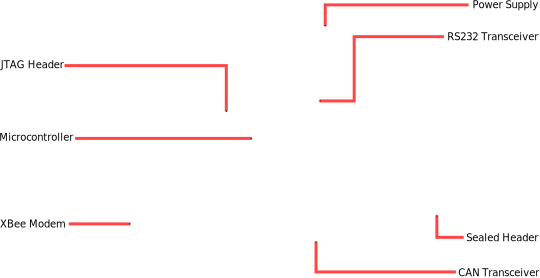
\includegraphics[scale=1]{implementation/figures/telemetry_pcb.eps}
\caption{Populated telemetry module PCB.}\label{fig:telemetry_pcb}
\end{figure}

\subsection{Hardware}

In addition to the base system hardware common to all modules described in Sec.\ \ref{sec:base_system_hardware}, several additional components were required in the implementation of the Telemetry module. A block diagram of the Telemetry module hardware implementation is shown in Fig.\ \ref{fig:telemetry_hardware_block}. The additional components are an XBee-PRO wireless mode, MAX232 RS-232 transceiver, MAX3100 external UART, an LTI1521 \unit{3.3}{\volt} linear voltage regulator, and an ST2378E 8-bit level translator. These additional components are listed in Table \ref{tab:telemetry_module_components} and will be described further in this chapter.

\begin{figure}[H]
\centering
\def\antenna{
  -- +(0mm,4.0mm) -- +(2.625mm,7.5mm) -- +(-2.625mm,7.5mm) -- +(0mm,4.0mm)
}

\begin{tikzpicture}[auto, node distance=4cm, draw=black!70, >=stealth']
  \node [block, name=max3100] {Max3100 SPI UART};
  \node [block, name=at90, right of=max3100] {AT90CAN};
  \node [block, name=rs232, right of=at90] {Max232 RS232 Transceiver};
  
  \node [block, name=can, below of=at90, above=1cm] {MCP2551 CAN Transceiver};
  \node [block, name=modem, left of=can] {XBee Modem};
  
  \node [block, name=ecu, right of=rs232] {ECU};
  \node [block, name=dac, below of=ecu, above=1cm] {DAC};

  \path (at90.north)+(0.0,+0.4) node (title) {Telemetry Module};

   \begin{pgfonlayer}{background}
       \path (max3100.north west)+(-0.3,0.7) node (a) {};
       \path (can.south -| rs232.east)+(+0.3,-0.2) node (b) {};
       \path[module] (a) rectangle (b);
   \end{pgfonlayer}

  \node [bus, name=can1, below of=can, label=below:CAN Bus, above=2.5cm] {CAN Bus};
  \node [bus, name=can2, left of=can1] {};
  \node [bus, name=can3, right of=can1] {};

  \draw [-, thick] (modem.west) -| ($(modem.west)+(-0.8,0.2)$) \antenna;

  \draw [-, line width=3pt] (can) -- (can1);
  \draw [-, line width=3pt] (can1) -- (can2);
  \draw [-, line width=3pt] (can1) -- (can3);

  \draw [<->, thick] (at90) -- node[] {SPI} (max3100);
  \draw [<->, thick] (max3100) -- node[text width=2cm] {Serial} (modem);
  \draw [<->, thick] ($(at90.east)+(0,0.1)$) to[myncbar, arm=1cm] ($(rs232.north west)+(0,-0.5)$);
  \draw [<-, thick] ($(at90.east)+(0,-0.1)$) to[myncbar, arm=1cm] ($(rs232.south west)+(0,+0.5)$);

  \draw [<->, thick] ($(rs232.north east)+(0,-0.5)$) to[myncbar, arm=1cm] (ecu);
  \draw [<-, thick] ($(rs232.south east)+(0,0.5)$) to[myncbar, arm=1cm] (dac);

  \draw [<->, thick] (at90) -- (can);

%  \draw [<->, thick] (modem) -- node[] {} (telemetry);
%  \draw [<->, thick] (telemetry) -- node[] {RS232} (ecu);
%  \draw [<->, thick] (telemetry) -- node[] {RS232} (daq);
%  \draw [-, thick] (modem) -- node[text width=1.5cm] {} (ant) \antenna;
\end{tikzpicture}
\caption{Block Diagram, Wireless Telemetry Module.\label{fig:telemetry_hardware_block}}
\end{figure}

\begin{table}[H]
  \caption{Wireless Telemetry Module Components\label{tab:telmetry_module_components}}
  \centering
    \begin{tabular}{|c|c|c|}
      \hline 
      Part & Manufacturer & Part Number\tabularnewline
      \hline
      \hline
      XBee-PRO OEM Module & Digi International & XBee-PRO\tabularnewline
      \hline 
      Dual RS-232 Transceiver & Maxim Electronics & MAX232\tabularnewline
      \hline 
      SPI-capable UART chip & Maxim Electronics & MAX3100\tabularnewline
      \hline 
      300mA Low Dropout Regulator & Linear Technology & LT1521\tabularnewline
      \hline
      8-bit dual-supply level translator & ST Microelectronics & ST2378E\tabularnewline
      \hline
    \end{tabular}
\end{table}

\subsubsection{Dual RS-232 Transceiver}

The ECU and the DAQ modules connect to the telemetry board with specialized cables that connect to the wiring harness. The ECU and DAQ interface with two built-in USART ports on the AT90CAN128 micro-controller. A MAX232 dual RS-232 trasceiver chip was used in the design to interface the built-in UARTS on the AT90CAN128 with the line levels expected by the serial ports on the ECU and DAQ.

\subsubsection{XBee-PRO Wireless Modem and External SPI UART}

To meet the range and data throughput requirements for the telemetry system, an XBee-PRO wireles modem was used. The XBee requires \unit{3.3}{\volt} I/O levels and power supply, and so a second linear voltage regulator was used in the design, the LT1521 from Linear Technology. Since the AT90CAN129 has only 2 built-in UARTS that were used for the RS232 interfaces to the ECU and DAQ, an third external UART was added to the design. The MAX3100 is a SPI-interfaced UART with an 8 word deep FIFO buffer. It is interfaced to the AT90CAN128's SPI pins and has an active-low IRQ line connected to external interrupt line EXT7 on the microcontroller.

The wireless transmitter consumes at most \unit{215}{\milli\ampere} of current during transmit \cite{XBeeManual}. Since the common module hardware only provides power for 5V devices, the telemetry module has a second LDO regulator providing \unit{3.3}{\volt}. A separate antenna port is connected to the modem and mounted in the side of the module enclosure.

Since the XBee, MAX3100, and AT90CAN128 are operating at different logic levels, a dual-supply level translator was used. Signals between the XBee, MAX3100, and the low supply voltage side of the level translator use \unit{+3.3}{\volt} logic, while signals between the AT90CAN128 and the high supply voltage side of the level translator use \unit{+5}{\volt} logic.

\subsection{Software}

The primary objective of the software running on the Telemetry Module is to push data around from various sources to various sinks. An overview of the Telemetry module's system software can be seen in Fig.\ \ref{fig:telemetry_software_implementation}. A layer of software drivers interacts directly with the hardware, providing an easy-to-use interface for the specific system software to use. Interrupt-driven USART drivers were written for the on-board USARTs of the AT90CAN128, as well as the MAX3100 external UART.

Three major libraries 

Nearly 3000 lines of c code were written by us for the Telemetry modules' system software. 3800 lines of code were also contributed by David Schilling for the DAC library.

\begin{figure}[H]
\centering
\begin{tikzpicture}[auto, node distance=2cm, draw=black!70, >=stealth']
%  \draw[help lines] (-3,-5) grid (8,2);
  
  % Usart0 section
  \node [blue shiny, rectangle, minimum width=2cm] (usart0) {UART0};
  \node [blue shiny, rectangle, above of=usart0, node distance=1cm] (ecu) {ECU};

  \node [red shiny, rectangle, below of=usart0, right=-1cm, node distance=1cm] (usart0_rx) {Rx};
  \node [red shiny, rectangle, below of=usart0, left=-1cm, node distance=1cm] (usart0_tx) {Tx};

  \draw [<->] (ecu) to (usart0);
  \draw [<-] (usart0_rx) -- ($(usart0.south west)!(usart0_rx.north)!(usart0.south east)$);
  \draw [->] (usart0_tx) -- ($(usart0.south west)!(usart0_tx.north)!(usart0.south east)$);
  
  % Max3100 section
  \node [blue shiny, rectangle, minimum width=2cm, right of=usart0, node distance=3cm] (max3100) {MAX3100};
  \node [blue shiny, rectangle, above of=max3100, node distance=1cm] (xbee) {Xbee};
  \node [blue shiny, rectangle, below of=max3100, above=-0.3cm, left=0.25cm, node distance=0, font=\tiny, inner sep=0.075cm] (max3100_rx_hw) {Rx};

  \node [red shiny, rectangle, below of=max3100, right=-1cm, node distance=1cm] (max3100_rx) {Rx};
  \node [red shiny, rectangle, below of=max3100, left=-1cm, node distance=1cm] (max3100_tx) {Tx};

  \draw [<->] (xbee) to (max3100);
  \draw [<-] (max3100_rx) -- ($(max3100_rx_hw.south west)!(max3100_rx.north)!(max3100_rx_hw.south east)$);
  \draw [->] (max3100_tx) -- ($(max3100.south west)!(max3100_tx.north)!(max3100.south east)$);

  \node [red shiny, rectangle split, rectangle split parts=3, below of=max3100, text width=1.8cm, font=\scriptsize, text centered,
	  minimum width=2cm, anchor=base] (xbee_library)
    {XBee Library
      \nodepart{second} Packetizer
      \nodepart{third} Packet Buffer};

  %\node [red shiny, rectangle, below of=packetizer, node distance=1cm, minimum width=2cm,
%	  text width=1.75cm, font=\scriptsize, text centered] (packet_buf) {Rx Packet Buffer};

  \draw [->] (max3100_rx) -- ($(xbee_library.north west)!(max3100_rx.south)!(xbee_library.north east)$);
  \draw [<-] (max3100_tx) -- ($(xbee_library.north west)!(max3100_tx.south)!(xbee_library.north east)$);

  % Usart1 section
  \node [blue shiny, rectangle, minimum width=2cm, right of=max3100, node distance=3cm] (usart1) {UART1};
  \node [blue shiny, rectangle, above of=usart1, node distance=1cm] (dac) {DAC};

  \node [red shiny, rectangle, below of=usart1, right=-1cm, node distance=1cm] (usart1_rx) {Rx};
  \node [red shiny, rectangle, below of=usart1, left=-1cm, node distance=1cm, dashed] (usart1_tx) {Tx};

  \draw [<->] (dac) to (usart1);
  \draw [<-] (usart1_rx) -- ($(usart1.south west)!(usart1_rx.north)!(usart1.south east)$);
  \draw [->, dashed] (usart1_tx) -- ($(usart1.south west)!(usart1_tx.north)!(usart1.south east)$);

  \node [red shiny, rectangle split, rectangle split parts=4, below of=usart1, text centered, minimum width=2cm, anchor=base, text width=1.85cm, inner xsep=0, font=\scriptsize] (dac_library)
    {DAC Library
      \nodepart{second} Buffer
      \nodepart{third} Decoder
      \nodepart{fourth} Encoder};

  \draw [->] (usart1_rx) -- ($(dac_library.north west)!(usart1_rx.south)!(dac_library.north east)$);
  \draw [<-, dashed] (usart1_tx) -- ($(dac_library.north west)!(usart1_tx.south)!(dac_library.north east)$);

  % CAN stuff
  \node [blue shiny, rectangle, minimum width=2cm, right of=usart1, node distance=3cm] (can) {CAN};
  \node [red shiny, rectangle, minimum width=2cm, below of=can, node distance=1cm] (can_driver) {Driver};

  \node at (dac_library.third split -| can_driver)
	    [red shiny, rectangle, minimum width=2cm, text width=1.85cm, font=\scriptsize, text centered] (can_library) {Telemetry CAN Library};

  \draw [<->] (can) -- (can_driver);
  \draw [<->] (can_driver) -- (can_library);

  \draw [->] (dac_library.third east) -- ($(can_library.north west)!(dac_library.third east)!(can_library.south west)$);
  \draw [<-] (dac_library.fourth east) -- ($(can_library.north west)!(dac_library.fourth east)!(can_library.south west)$);

  % Now for the rest of the connections
  \draw [->] (xbee_library.third west) -| (usart0_tx);
  \draw [<-] (xbee_library.second west) -| (usart0_rx);
  \draw [->] (dac_library.second west) to node [name=mid1] {} (xbee_library.second east);
  \draw [->] (dac_library.fourth west) -| (mid1);

  \node [left of=usart0, node distance=3cm, minimum width=3.5cm] (perifs) {Module Periferals};
  \node [below of=perifs, node distance=1cm, minimum width=3.5cm] (buffers) {Drivers/Buffers};
  \node [below of=buffers, node distance=1cm, minimum width=3.5cm] (libraries) {Libraries};

  \begin{pgfonlayer}{background}
    \path (perifs.north west)+(-0.0,0.1) node (a1) {};
    \path (can.south east)+(+0.1,-0.1) node (b1) {};
    \path[draw=blue!50!black!50, rounded corners=0.1cm] (a1) rectangle (b1);

    \path (buffers.north west)+(-0.0,0.1) node (a2) {};
    \path (can_driver.south east)+(0.1,-0.1) node (b2) {};
    \path [draw=red!50!black!50, rounded corners=0.1cm] (a2) rectangle (b2);

    \path (libraries.north west)+(-0.0,0.1) node (a3) {};
    \path (can_library.south east)+(0.1,-0.1) node (b3) {};
    \path [draw=red!50!black!50, rounded corners=0.1cm] (a3) rectangle (b3);
  \end{pgfonlayer}

  % Guide
  \node at ($(a3 |- b3)+(0.0,-0.1)$) [anchor=north west, blue shiny, minimum width=2cm] (hardware) {Hardware};
  \node [red shiny, right of=hardware, node distance=2.2cm, minimum width=2cm] (software) {Software};
  
\end{tikzpicture}

\caption{Telemetry software overview.}
\label{fig:telemetry_software_implementation}
\end{figure}

\subsubsection{Internal and External USART Drivers}

Software drivers for both the internal built-in USART periferals as well as the MAX3100 external UART were written in a similar fashion, and share the same software interfaces and buffering code. The drivers were written to utilize the hardware interrupts of the periferals to allow asynchronous sending and receiving of data. A statically allocated circular buffering approach was taken for both receiving and transmitting data. An abstracted flow chart of the USART interrupt handling is shown in Fig.\ \ref{fig:usart_driver_flow}.

\paragraph{MAX3100 SPI Interface}

The datahseet for the MAX3100 states that the minimum SPI Clock period is $t_{CP}=\unit{238}{\nano\second}$, which results in a maximum frequency of approximately $\unit{4.2}{\mega\hertz}$ \cite{MAX3100}. The SPI periferal was thus set to use 1/4 of the system clocks frequency resulting in $\unit{4}{\mega\hertz}$.

\begin{figure}[H]
\centering
\begin{tikzpicture}[auto, node distance=2cm, draw=black!70, >=stealth']
  \node [start] (int) {Interrupt};
  \node [decision, right of=int, right=0cm] (rx) {Rx Byte?};
  \node [block, below of=rx] (add) {Add to Rx buf.};

  \node [decision, right of=rx, right=0cm] (tx) {Tx Byte?};
  \node [block, below of=tx, text width=2.5cm, inner xsep=0pt] (remove) {Remove from Tx buf.};
  \node [end, right of=tx, right=0cm] (return) {Return};

  \draw [->] (int) -- (rx);
  \draw [->] (rx) to node [] {yes} (add);

  \draw [->] (rx) -- node [name=mid] {no} (tx);
  \draw [->] (add) -| (mid);

  \draw [->] (tx) to node [] {yes} (remove);
  \draw [->] (tx) -- node [name=mid2] {no} (return);
  \draw [->] (remove) -| (mid2);

\end{tikzpicture}
\caption{Basic USART interrupt flow diagram.}
\label{fig:usart_driver_flow}
\end{figure}

\subsubsection{Xbee Library}

In order to facilitate routing data to and from multiple sources and sinks, it was determined that the Xbee would need to be interfaced using the special "API" mode described in the Xbee documentation \cite{XBeeManual}. The API mode is characterized by a packet interface that needed to be implemented in software. A library was written to implement two critical pieces of functionality:

\begin{enumerate}
\item to set the modem into API mode operation and manage the modem's operating state;
\item and to send and receive packetized data from the modem on behalf of the user software as per the Xbee's API specification \cite{XBeeManual};
\end{enumerate}

The Xbee library implements the binary packet protocol described in the XBee manual, and is able to send and receive unicast and multicast packets. The driver is only capable of sending packets to 16-bit addresses. Full 64-bit address mode was not implemented as the address space was not required in our 3 node network. The driver is also capable of sending command-type packets to the modem and reading the response.

Managing the modem's state was implemented as a state machine. Since minimal functionality was required, only a handful of modem commands were implemented. The driver is able to push the modem into API mode, after which all communication is done using the packet interface.

The modem commands implemented are listed in Table \ref{tab:xbee_commands}.

\begin{table}
\caption{Implemented Xbee modem commands.\label{tab:xbee_commands}}
\centering{}
\begin{tabular}{|l|l|}
\hline 
Command & Description \tabularnewline
\hline
\hline
AP & Set and read the API mode state \tabularnewline
\hline
CH & Set and read the RF channel \tabularnewline
\hline 
ID & Set and read the PAN (Personal Area Network) ID \tabularnewline
\hline
MY & Set and read the modems local address \tabularnewline
\hline
\end{tabular}
\end{table}

Similar to the rest of the software drivers implemented, the Xbee library uses callbacks to provide the user software with incoming data. Function pointers are used to connect the library to a UART, which makes it possible to reconfigure the library to use a different USART on-the-fly.

\subsubsection{DAC Library}

To reduce the implementation work required by us, we asked David Schilling, a computer science student on the Formula SAE team, to write the DAC software library to read and write the DAC's serial format, given the requirements described in Section \ref{sec:Telemetry-Module-Design}.

The DAC library maintains it's own buffer of incoming DAC data. We also asked Dave to provide seperate functions for buffering incoming data, and for processing that data. This seperation allowed the library to be easily tied in with the rest of the system software on the telemetry module: adding a data to the DAC buffer occurs whenever the internal USART driver interrupts with a new byte, and processing is called from the mainline loop.

\subsubsection{Main Control Loop}